
\documentclass[12pt]{article}
\usepackage{amsmath,amssymb,bm}
\usepackage{geometry}
\geometry{margin=1in}
\usepackage{siunitx}
\sisetup{detect-all=true}
\usepackage{tikz}
\usetikzlibrary{arrows.meta,positioning,fit,shapes.geometric}

\title{Appendix M -- Energy and Safety Limits for UBT Experiments}
\date{}

\begin{document}
\maketitle

\section*{M.1 Purpose}
This appendix specifies energetic and safety envelopes for laboratory tests of Unified Biquaternion Theory (UBT) using standing/modulated EM modes (cf.\ Appendix L) and their phase-sector coupling through $\psi$. Where $\psi\!=\!0$ (or averages to zero), UBT reduces to GR/Maxwell and remains consistent with existing experiments.

\section*{M.2 Scaling Relations (Stored Energy, Drive Power)}
For a cavity mode with angular frequency $\omega=2\pi f$, volume $V$, effective permittivity $\epsilon_{\rm eff}$, rms electric field $E_{\rm rms}$ and quality factor $Q$,
\begin{equation}
U \;\approx\; \tfrac{1}{2}\,\epsilon_{\rm eff}\,E_{\rm rms}^2\,V,\qquad
P_{\rm in} \;\approx\; \frac{\omega\,U}{Q}.
\end{equation}
The fractional frequency shift of a metrological probe by a weak metric perturbation $h_{\mu\nu}$ is
\begin{equation}
\frac{\Delta f}{f}\;\simeq\; -\frac{1}{2}\,\big\langle h_{00}+n^i n^j h_{ij}\big\rangle_{\rm mode},
\end{equation}
with $n^i$ the local propagation direction. In GR alone, EM $T^{\mu\nu}$ yields negligibly small $h_{\mu\nu}$ for lab powers; in UBT, the effective source is
\begin{equation}
T^{\mu\nu}_{\rm eff} \;=\; T^{\mu\nu}_{\rm EM} + \lambda_\psi\,\Psi^{\mu\nu}(\psi,F) \quad\Rightarrow\quad
h_{\mu\nu}\propto \int \! \frac{T^{\mu\nu}_{\rm eff}}{|\mathbf{x}-\mathbf{x}'|}\,d^3x' \;\;(\text{Appendix L}).
\end{equation}

\section*{M.3 Numeric Envelope (Indicative Values)}
Assuming $V=\SI{1.0e-3}{m^3}$, $Q=10^6$, $\epsilon_{\rm eff}\approx \epsilon_0$, two drive levels give:
\begin{center}\small
\begin{tabular}{|c|c|c|c|}
\hline
$f$ [GHz] & $E_{\rm rms}$ [kV/m] & $U$ [J] & $P_{\rm in}$ [W] \\ \hline
2.4 & 50  & 0.011 & 0.17 \\
5.0 & 50  & 0.011 & 0.35 \\
10.0& 50  & 0.011 & 0.70 \\ \hline
2.4 & 200 & 0.18  & 2.7  \\
5.0 & 200 & 0.18  & 5.7  \\
10.0& 200 & 0.18  & 11.3 \\ \hline
\end{tabular}
\end{center}
These are order-of-magnitude targets; thermal management and breakdown thresholds must be respected (Sec.\ M.5).

\section*{M.4 Detectability Window}
Let $\Delta f/f \ge \sigma_f$ be the instrument sensitivity (e.g.\ $\sigma_f\sim 10^{-8}$). Writing
\begin{equation}
\frac{\Delta f}{f} \;\sim\; \mathcal{K}_{\rm UBT}\, U \,,
\end{equation}
the minimum stored energy is $U_{\min}\approx \sigma_f/\mathcal{K}_{\rm UBT}$. In GR one expects $\mathcal{K}_{\rm GR}\!\ll\!\mathcal{K}_{\rm UBT}$; thus any detection at lab powers constrains $\lambda_\psi$ and $\Psi^{\mu\nu}$.

\section*{M.5 Safety Limits}
\begin{itemize}
\item \textbf{Dielectric breakdown (vacuum)}: avoid peak fields $\gtrsim \SI{30}{MV/m}$ at surfaces; smooth geometry, proper conditioning.
\item \textbf{Heating/Quench}: keep surface losses below cryostat capacity; derate for seams and couplers.
\item \textbf{Exposure/EMC}: enclose in Faraday cage; comply with local RF exposure limits; interlocks and E-stop required.
\end{itemize}

\section*{M.6 Control and Modulation of Hopfions \& Psychons}
UBT links hopfion topology and psychon excitations through the phase sector $\psi$. A practical loop: EM field pattern $\to T^{\mu\nu}_{\rm eff}\to \Delta g_{\mu\nu}$, while $\psi$ modulates both $T^{\mu\nu}_{\rm eff}$ and the metric response (Appendix L). Below is a \emph{self-contained TikZ} block diagram (no external file).

\begin{figure}[h!]
\centering
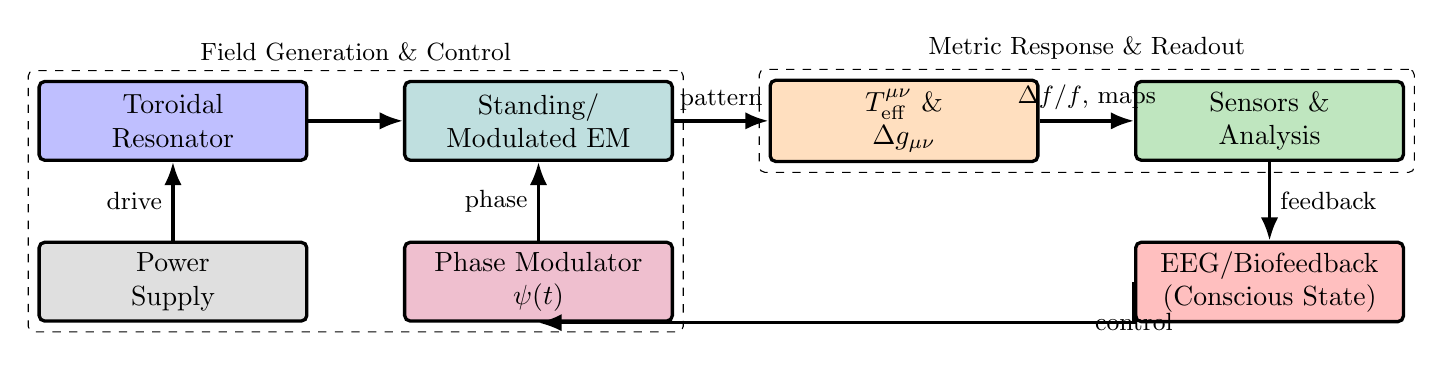
\begin{tikzpicture}[
  node distance=10mm and 12mm,
  box/.style={draw, rounded corners=2pt, very thick, align=center, minimum width=34mm, minimum height=10mm, fill=#1!25},
  arr/.style={-Latex, very thick},
  note/.style={font=\small, align=center}
]
% Nodes
\node[box=blue]   (res) {Toroidal\\Resonator};
\node[box=teal, right=of res] (em) {Standing/\\Modulated EM};
\node[box=purple, below=of em] (psi) {Phase Modulator\\$\psi(t)$};
\node[box=gray, below=of res] (psrc) {Power\\Supply};
\node[box=orange, right=of em] (metric) {$T^{\mu\nu}_{\rm eff}$ \&\\$\Delta g_{\mu\nu}$};
\node[box=green!60!black, right=of metric] (sense) {Sensors \&\\Analysis};
\node[box=red, below=of sense] (bio) {EEG/Biofeedback\\(Conscious State)};

% Arrows
\draw[arr] (psrc) -- (res) node[midway,left,note]{drive};
\draw[arr] (res) -- (em);
\draw[arr] (psi) -- (em) node[midway,left,note]{phase};
\draw[arr] (em) -- (metric) node[midway,above,note]{pattern};
\draw[arr] (metric) -- (sense) node[midway,above,note]{$\Delta f/f$, maps};
\draw[arr] (sense) -- (bio) node[midway,right,note]{feedback};
\draw[arr] (bio.west) |- (psi.south) node[pos=0.25,below,note]{control};

% Fit boxes (labels)
\node[draw,dashed,rounded corners=2pt,fit=(res)(em)(psrc)(psi),label=above:{\small Field Generation \& Control}] {};
\node[draw,dashed,rounded corners=2pt,fit=(metric)(sense),label=above:{\small Metric Response \& Readout}] {};

\end{tikzpicture}
\caption{Closed-loop control of hopfion/psychon dynamics via phase modulation $\psi(t)$ and standing/modulated EM fields. Diagram is drawn with TikZ (no external image).}
\label{fig:M_loop}
\end{figure}

\section*{M.7 Summary}
UBT-compatible operation keeps EM powers in safe ranges while seeking a measurable metrological signature ($\Delta f/f$) mediated by the $\psi$-sector. The TikZ control diagram specifies a practical loop for hopfion/psychon modulation without external figures.

\end{document}
